\chapter{Einleitung}

\section{Aufgabenbeschreibung}

Ziel dieses Semesterprojekts ist es mit Rhapsody, einem mächtigem Tool zur Codegenerierung, Design Patterns zu implementieren. Diese werden standardmäßig von Rhapsody nicht angeboten und sollen in Form von Stereotypen während diesem Semester implementiert und getestet werden. \\
\\
In dem vorangegangenen Semester wurde die Umsetzbarkeit der Design Pattern Singleton und Observer belegt. Weiterhin soll das Design Pattern Guarded Call umgesetzt werden. \\
Diese sollen nun dieses Semester vollständig umgesetzt und getestet werden. Sind diese Stereotypen dann vollständig in Rhapsody implementiert, soll Rhapsody automatisch Java-Klassen aufrufen, welche dann das als Objektbaum vorliegende Modell umbauen können.\\

\begin{figure}[!htbp]
	\centering
	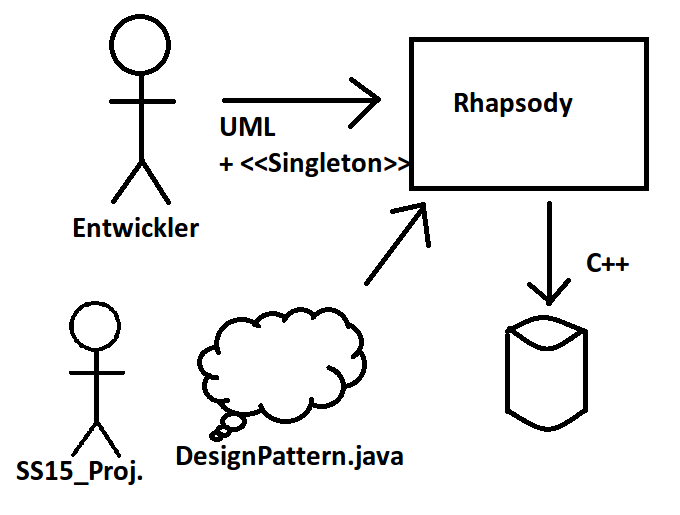
\includegraphics[width=0.66\textwidth]{content/pictures/Simplification}
	\label{pic:bild}
	\caption{Ein Diagramm der Nutzung der Umsetzung der Design Patterns}
\end{figure}

Die enstprechenden Design Patterns werden im Laufe der Dokumentation genauer erläutert.\\
Das Projekt umfasst hierbei nicht nur die Implementierung der Design Patterns für Rhapsody, sondern auch das Schreiben einer Anwenderdokumentation, das Erstellen von Testfällen und letztlich das Durchführen der Tests. Im Folgenden werden diese Phasen genauer erläutert.

\section{Implementierung}

Die Implementierung, welche insgesamt nur einen Umfang von 30-40 \% der Gesamtzeit des Projekts in Anspruch nehmen soll, umfasst das Umsetzen der drei Design Patterns für Rhapsody, sodass ein Programmierer, der Rhapsody nutzt, in Zukunft nur ein UML-Diagramm seines Projekts eingeben und die entsprechenden Stereotypen auswählen muss, um sein Projekt mit Design Patterns auszustatten. Um die Implementierung der Muster muss er sich in Zukunft also keine Gedanken mehr machen, diese Aufgabe übernimmt in Zukunft Rhapsody.\\
Die Umsetzung der Patterns erfolgt über eine Datei “DesignPatterns.java”, die beim Erstellen eines Projekts mit Stereotypen von Rhapsody aufgerufen wird. In ihr definieren wir die Design Patterns für C++ so, dass sie in bestehende Projekte eingearbeitet werden können.

\section{Anwenderdokumentation/Handbuch}

Die Anwenderdokumentation bzw. das Handbuch soll zeitlich am Anfang des Projekts fertiggestellt werden. In ihr werden zukünftigen Nutzern Anwendungsfälle und Vorgehensweisen erläutert. Zum einen soll das Handbuch eine Hilfe für die Nutzer des Projektes werden, zum anderen stellt es den Grundstein für die Erstellung von Testfällen dar. Nur wenn die Anwendungsfälle vollständig und korrekt beschrieben werden, können davon sinnvolle Testfälle abgeleitet werden.\\
Daher ist die Erstellung des Handbuchs eine Aufgabe, die zeitlich am Anfang des Projekts angesiedelt ist.

\section{Simplification}
Der \textit{Simplification-Prozess} wird von Rhapsody übernommen und transformiert die
erzeugten UML-Diagramme in Code. Anhand von verschiedenen Ablaufdiagrammen kann
auch gleich das Verhalten spezifiziert werden. So lassen sich leicht und schnell
lauffähige Programme erstellen.\\
\newline
Da Rhapsody leider keine Möglichkeit bietet, verschiedene Design Pattern
\enquote{von Haus aus} einzubinden, müssen wir dies manuell tun. Wir greifen in
den Simplification-Prozess ein und zwingen Rhapsody manuell unsere Implementierung
zu verwenden.\\
Hierfür greift der Code-Generator auf den vom Benutzer eingestellten Helper zu.
Hier werden die erzeugten Java-Klassen eingebunden und verarbeitet. Diese
erzeugen dann die Simplification-Klassen Singleton, Observer und Guarded Call.
Damit Rhapsody unsere User-Simplification verwendet muss in den \textit{Simplify
Properties} eingestellt werden, dass unser User Simplifier benutzt werden soll.
\cite{oldDoku}

\begin{figure}[!htbp]
	\centering
	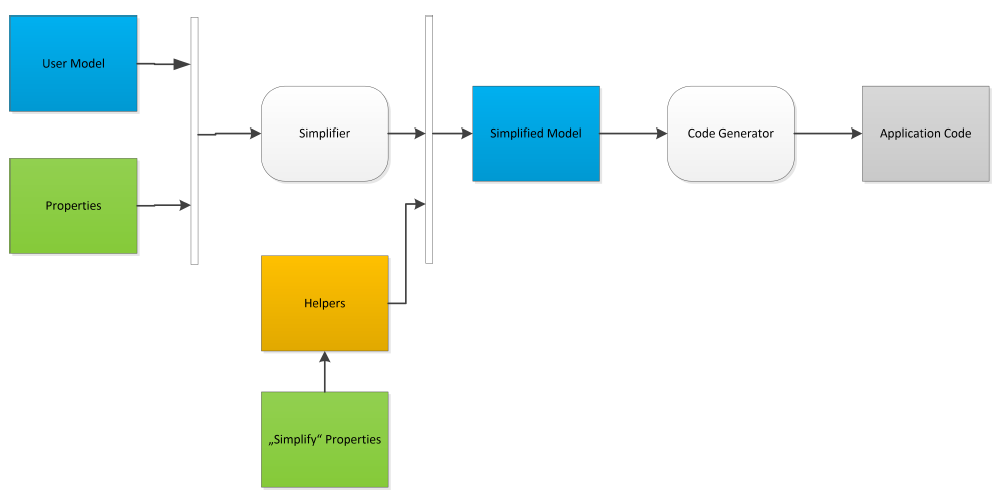
\includegraphics[width=0.99\textwidth]{content/pictures/simplifier.png}
	\label{pic:bild}
	\caption{Simplification Ablauf \cite{oldDoku}}
\end{figure}

Damit Rhapsody weiß wo diese Java-Klassen liegen, muss man die \enquote{.hep} Datei
anpassen. Diese befindet sich in unserem Fall unter dem jeweiligen
Benutzer/IBM/\ldots/HFUSingletonPattern/model/HFUSingletonPattern_rpy. Hier ist
die gesuchte .hep Datei.
 
\begin{figure}[!htbp]
	\centering
	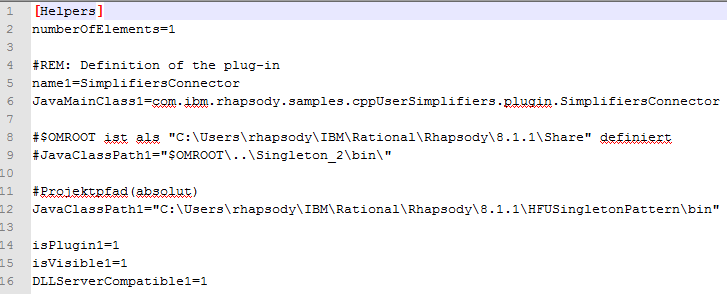
\includegraphics[width=0.99\textwidth]{content/pictures/hep.png}
	\label{pic:bild}
	\caption{Inhalt der .hep Datei}
\end{figure} 

\textbf{Wichtig:} bei Änderungen in der Datei sollte Rhapsody neu gestartet
werden. Hier ist das Problem das Rhapsody den Cache erst leeren muss und dies
erfolgt leider nur nach einem Neustart. 
\section{Testen}

Das Testen ist der wichtigste und größte Teil des Projektes. Nachdem das Handbuch fertig
geschrieben und somit die Anwendungsfälle definiert wurden, müssen dazu passende Testfälle
entworfen werden. Aufgrund der vielen Unbekannten, die aus einem Projekt entstehen können,
gibt es viele potentielle Fehlerquellen, die abgedeckt werden müssen. Nur wenn alle Tests 
bestanden werden gilt das Projekt als erfolgreich.\\
Für die Durchführung gilt: Die Gruppe, die die Beschreibung verfasst hat,
schreibt auch die jeweiligen Testfälle dazu. Die andere Gruppe kümmert sich um die
Implementierung der Design Pattern. So wird überprüft, ob die Beschreibung auch
wirklich vollständig ist. Gleichzeitig wird so die Qualität der Anwendungs- und
der daraus abgeleiteten Testfälle deutlich.\\
Für Testfälle, die nicht erfolgreich durchgeführt werden, ist am Ende des Projektzeitplans
ein kurzer Korrekturzeitraum eingeplant. 